%15 min preso!
\documentclass[xcolor=table,aspectratio=169]{beamer}
\usepackage{beamerthemesplit}
\usepackage{wrapfig}
\usetheme{SPbGU}
\usepackage{pdfpages}
\usepackage{amsmath}
\usepackage{cmap}
\usepackage[T2A]{fontenc}
\usepackage[utf8]{inputenc}
\usepackage[english]{babel}
\usepackage{indentfirst}
\usepackage{amsmath}
\usepackage{tikz}
\usepackage{multirow}
\usepackage[noend]{algpseudocode}
\usepackage{algorithm}
\usepackage{algorithmicx}
\usepackage{fancyvrb}
\usepackage{hyperref} 
\usetikzlibrary{calc}
\usetikzlibrary{shapes}
\usetikzlibrary{arrows,automata}
\usetikzlibrary{positioning}
\usetikzlibrary{fit}
\usetikzlibrary{shapes.callouts}
\usetikzlibrary{shapes.misc}
\usepackage{xparse}

\usepackage{etoolbox,refcount}
\usepackage{multicol}

\usepackage{fontawesome5}
\usepackage{fontawesome}

\usepackage{tabularx}
\newcolumntype{Y}{>{\raggedleft\arraybackslash}X}

\renewcommand{\thealgorithm}{}

\newtheorem{mytheorem}{Theorem}
\renewcommand{\thealgorithm}{}

\newcommand{\tikzmark}[1]{\tikz[overlay,remember picture] \node (#1) {};}
\def\Put(#1,#2)#3{\leavevmode\makebox(0,0){\put(#1,#2){#3}}}

\newcommand{\ltz}{$< 1$}

\tikzset{
    state/.style={
           rectangle,
           rounded corners,
           draw=black, very thick,
           minimum height=2em,
           inner sep=2pt,
           text centered,
           },
}

\tikzset{
    invisible/.style={opacity=0,text opacity=0},
    visible on/.style={alt=#1{}{invisible}},
    alt/.code args={<#1>#2#3}{%
      \alt<#1>{\pgfkeysalso{#2}}{\pgfkeysalso{#3}} % \pgfkeysalso doesn't change the path
    },
}

\tikzset{cross/.style={cross out, draw=black, minimum size=2*(#1-\pgflinewidth), inner sep=0pt, outer sep=0pt, ultra thick},
%default radius will be 1pt. 
cross/.default={1pt}}

\NewDocumentCommand{\mycallout}{r<> O{opacity=0.8,text opacity=1} m m m}{%
\tikz[remember picture, overlay]\node[align=center, fill=cyan!20, text width=#5cm,
#2,visible on=<#1>, rounded corners,
draw,rectangle callout,anchor=pointer,callout relative pointer={(290:0.5cm)}]
at (#3) {#4};
}

\NewDocumentCommand{\mycalloutR}{r<> O{opacity=0.8,text opacity=1} m m m}{%
\tikz[remember picture, overlay]\node[align=center, fill=cyan!20, text width=#5cm,
#2,visible on=<#1>, rounded corners,
draw,rectangle callout,anchor=pointer,callout relative pointer={(30:0.8cm)}]
at (#3) {#4};
}


%callout relative pointer={(230:0.5cm)}]

\newcounter{countitems}
\newcounter{nextitemizecount}
\newcommand{\setupcountitems}{%
  \stepcounter{nextitemizecount}%
  \setcounter{countitems}{0}%
  \preto\item{\stepcounter{countitems}}%
}
\makeatletter
\newcommand{\computecountitems}{%
  \edef\@currentlabel{\number\c@countitems}%
  \label{countitems@\number\numexpr\value{nextitemizecount}-1\relax}%
}
\newcommand{\nextitemizecount}{%
  \getrefnumber{countitems@\number\c@nextitemizecount}%
}
\newcommand{\previtemizecount}{%
  \getrefnumber{countitems@\number\numexpr\value{nextitemizecount}-1\relax}%
}
\makeatother    
\newenvironment{AutoMultiColItemize}{%
\ifnumcomp{\nextitemizecount}{>}{3}{\begin{multicols}{2}}{}%
\setupcountitems\begin{itemize}}%
{\end{itemize}%
\unskip\computecountitems\ifnumcomp{\previtemizecount}{>}{3}{\end{multicols}}{}}


\beamertemplatenavigationsymbolsempty

\title[Modern Parsing Techniques]{Modern Parsing Techniques}
\subtitle{All You Need is Generalized GLL}
%\institute[PL\&T@SPbSU]{
%Saint Petersburg State University
%}

% То, что в квадратных скобках, отображается в левом нижнем углу.
\author[Semyon Grigorev]{Semyon Grigorev}

%\date{September 26, 2022}

\begin{document}
{
\begin{frame}[fragile]
  %\begin{table}
  %\centering
  %
\includegraphics[height=1.5cm]{pictures/SPbGU_Logo.png}  
  %\end{table}
  \titlepage
\end{frame}
}


% LL
% Combinators, left recursive productions
% ANTLR
% TreeSitter
% Iguana
% GLL
% Error recovery
% Incremental parsing
% Code generation
% Scanerless
% PEG -> GLL
% String-embedded languages processing


\begin{frame}[fragile]
  \frametitle{Parsing: Problems and Challenges}  
  \tikzset{dbl/.style={double,double distance=2pt}} 
  \begin{minipage}[t]{0.49\textwidth}
    Language specification approaches Zoo
    \begin{itemize}
      \item Lexer + Parser vs Scannerless: grammar over tokens vs grammar over characters 
      \item Context-free grammars (CFG): BNF, EBNF, ...      
      \item Data-dependent grammars: utilization of previously parsed data to guide parsing
      \item Rail diagrams: graphical language
      \item Parsing Expression Grammars (PEG): CFG with prioritized choice and manual control of lookahead  
      \item \ldots
    \end{itemize}
  \end{minipage}  
  \begin{minipage}[t]{0.49\textwidth}
    Language/grammar properties
    \begin{itemize}
      \item Determinism and ambiguity
      \item (Hidden) Left recursion
      \item \ldots
    \end{itemize}
    Technical challenges
    \begin{itemize}
      \item Performance
      \item Error recovery
      \item Incremental parsing
      \item Manual control of behavior
    \end{itemize}
  \end{minipage}
\end{frame}

\begin{frame}[fragile]
  \frametitle{ANTLR}  
  \begin{minipage}[t]{0.48\textwidth}
  \begin{itemize}
    \item \href{https://www.antlr.org/papers/allstar-techreport.pdf}{Adaptive LL(*) Parsing: The Power of Dynamic Analysis}
    \item ALL(*)
    \item \href{https://github.com/antlr/grammars-v4}{Huge grammar zoo}
    \item Can generates parser in Java, C\#, Python, JavaScript, Go, C++, Swift, Dart, PHP
    \item[\faPlus] Simple error recovery
    \item[\faPlus] Left recursion
    \item[\faPlus] Prioritized choice
    \item[\faPlus] Parsing tree and visitors, listeners for it
  \end{itemize}
\end{minipage}
\begin{minipage}[t]{0.48\textwidth}
  \begin{figure}
    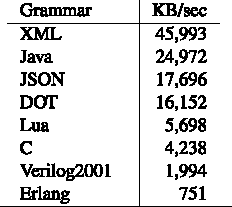
\includegraphics[width=0.8\textwidth]{pictures/antlrPerformance.pdf}
    \caption{Throughput of lexing+parsing; all input preloaded into RAM\footnotemark}
  \end{figure}
\end{minipage}
\footnotetext{From ``Adaptive LL(*) Parsing: The Power of Dynamic Analysis''}
\end{frame}

\begin{frame}[fragile]
  \frametitle{Iguana}
  \begin{minipage}[t]{0.48\textwidth}
    
  
    \begin{itemize}
      \item GLL-based
      \item \href{https://github.com/iguana-parser/iguana}{Sources}
      \item \href{https://www.cwi.nl/nieuws/2019/thesis_final-1.pdf}{Practical General Top-Down Parsers}
      \item[\faPlus] \href{Semantics and Algorithms for Data-dependent Grammars}{Data-dependent grammars}
      \item[\faPlus] Left recursion
      \item[\faPlus] Prioritized choice
      \item[\faPlus] Operator associativity 
      \item[\faPlus] Layout rules    
    \end{itemize}  
  \end{minipage}  
  \begin{minipage}[t]{0.48\textwidth}
    \begin{figure}
      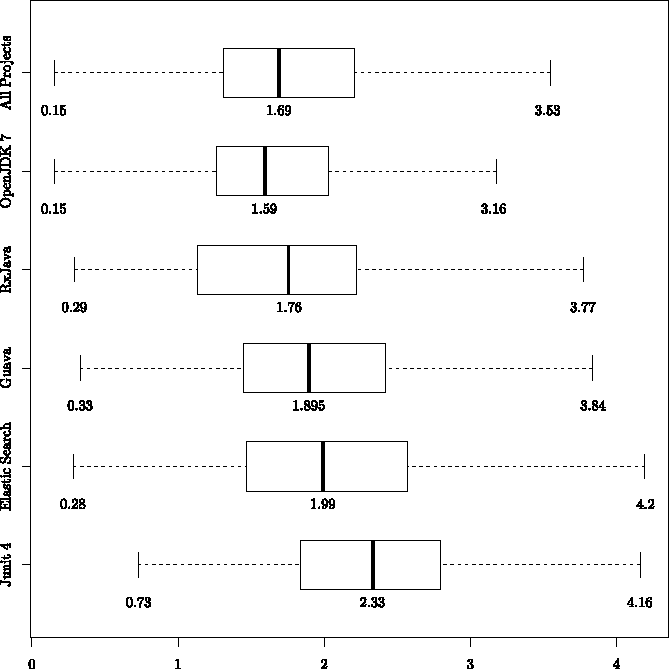
\includegraphics[width=0.7\textwidth]{pictures/IguanaPerformance.pdf}
      \caption{Iguana performance relative ot ANTLR\footnotemark}
    \end{figure}
  \end{minipage}
  \footnotetext{From ``Practical General Top-Down Parsers''}
\end{frame}

\begin{frame}[fragile]
  \frametitle{Tree-Sitter}
  \begin{itemize}
    \item GLR-based
    \item \href{https://github.com/tree-sitter/tree-sitter}{Sources}
    \item[\faPlus] Huge grammar zoo
    \item[\faPlus] Incremental
    \item[\faPlus] Error recovery
    \item[\faPlus] Operators precedence  and associativity
    \item[\faMinus] Custom lexers to handle layout
    \item[\faMinus] Parsers in C with bindings to other languages  
    \item[\faMinus] Prioritized choice 
  \end{itemize}    
\end{frame}


\begin{frame}[fragile]
  \frametitle{SDF3 (Spoofax)}
  \begin{itemize}
    \item GLR-based
    \item[\faPlus] Modular
    \item[\faPlus] Layout rules
    \item[\faPlus] Operators associativity
    \item[\faMinus\faQuestion] Error recovery
    \item Incremental version under development\footnote{\href{https://dl.acm.org/doi/abs/10.1145/3359061.3361085}{Incremental scannerless generalized LR parsing}}
  \end{itemize}  
  
  \begin{itemize}
    \item Part of \href{https://www.spoofax.dev/}{Spoofax language workbench}
    \item \href{https://github.com/metaborg/sdf}{Sources}
    \item \href{https://www.spoofax.dev/references/syntax/}{Documentation}
    \item \href{https://link.springer.com/chapter/10.1007/978-3-030-58768-0_1}{Multi-purpose Syntax Definition with SDF3}
  \end{itemize}  
  
\end{frame}


\begin{frame}[fragile]
  \frametitle{Parser combinators}  
  \begin{itemize}
    \item[\faThumbsODown] Poor performance 
    \item[\faTimes] Left recursion
    \item[\faTimes] Ambiguity 
    \item[\faTimes] Error recovery
    \item[\faTimes] Incremental parsing  
    
    \item[\faLightbulbO] Modern combinator library is not just a set of functions
    \begin{itemize}
      \item[\faThumbsOUp] Good performance
      \item[\faPlus] Left recursion 
      \item[\faPlus] Ambiguity
      \item[\faQuestion] Error recovery
      \item[\faQuestion] Incremental parsing
      \item[\faThumbsODown] You have no control on nontrivial machinery inside
    \end{itemize}
  \end{itemize}
\end{frame}


\begin{frame}[fragile]
  \frametitle{Parsley}  
  \begin{figure}
    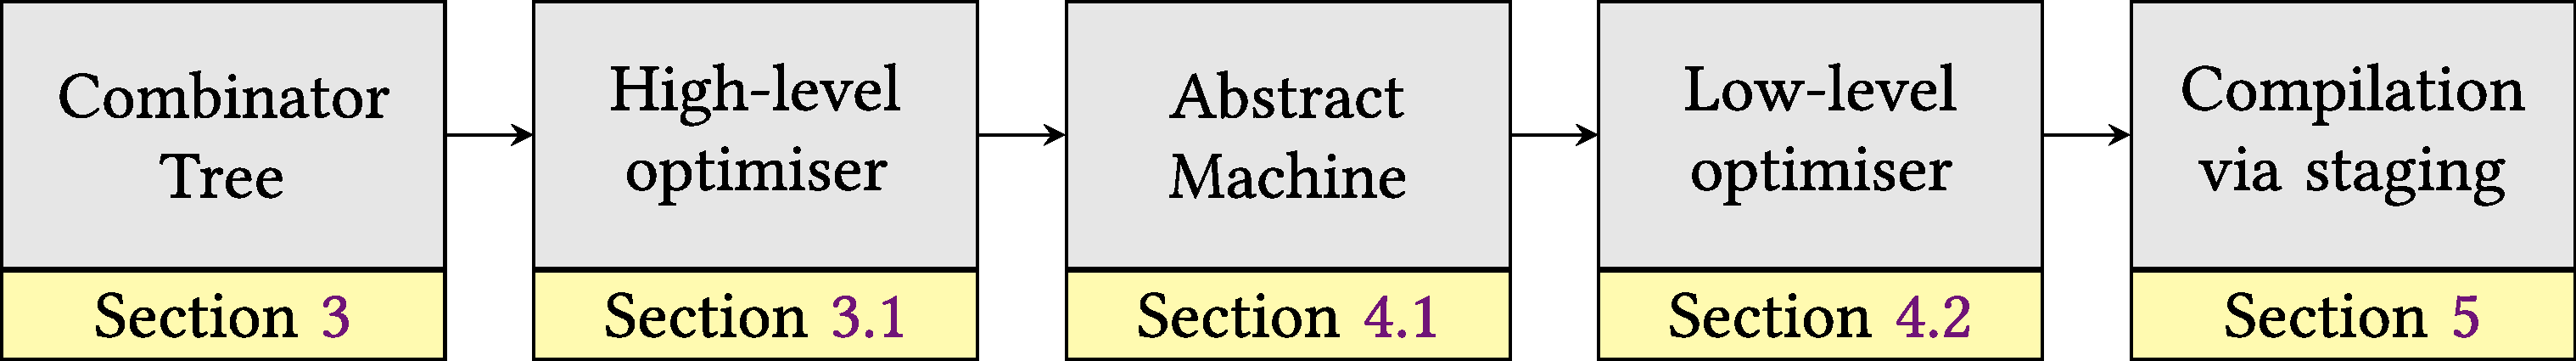
\includegraphics[width=0.9\textwidth]{pictures/ParsleyArch.pdf}
    \caption{Parsley internal pipeline\footnote{From ``Staged Selective Parser Combinators''}}  
  \end{figure}
  \begin{figure}
    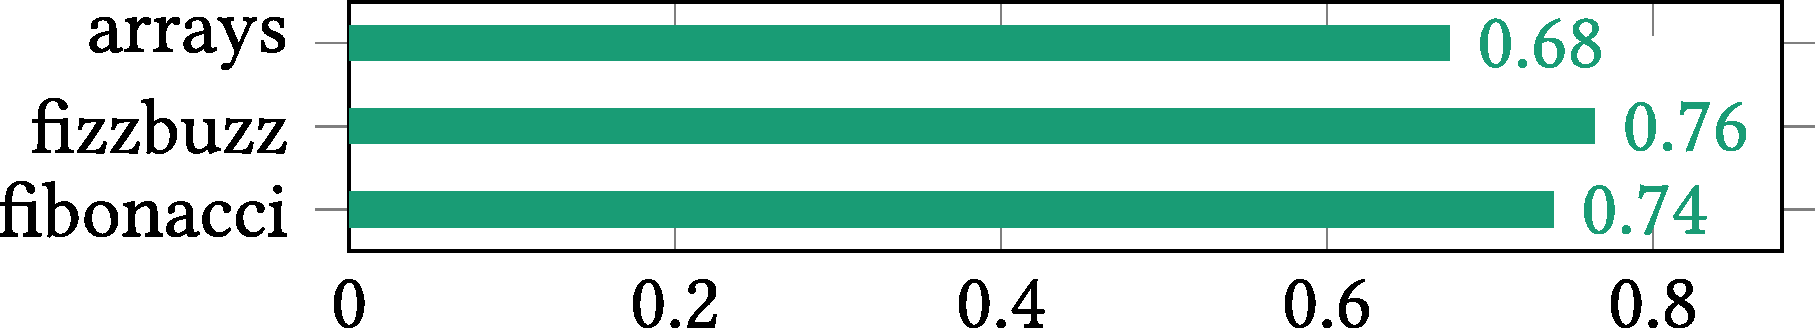
\includegraphics[width=0.8\textwidth]{pictures/ParsleyBison.pdf}
    \caption{Parsley performance relative to Bison\footnote{From ``Staged Selective Parser Combinators''}}  
  \end{figure}
\end{frame}

\begin{frame}[fragile]
  \frametitle{Meerkat}
  \begin{minipage}[t]{0.4\textwidth}
  \begin{itemize}
    \item GLL-like engine for CPS parsers
    \item \href{https://dl.acm.org/doi/10.1145/2847538.2847539}{Practical, general parser combinators}
    \item[\faPlus] Left recursion
    \item[\faPlus] Prioritized choice
    \item[\faPlus] Operator associativity 
  \end{itemize} 
\end{minipage}  
  \begin{minipage}[t]{0.58\textwidth}
    \begin{figure}
      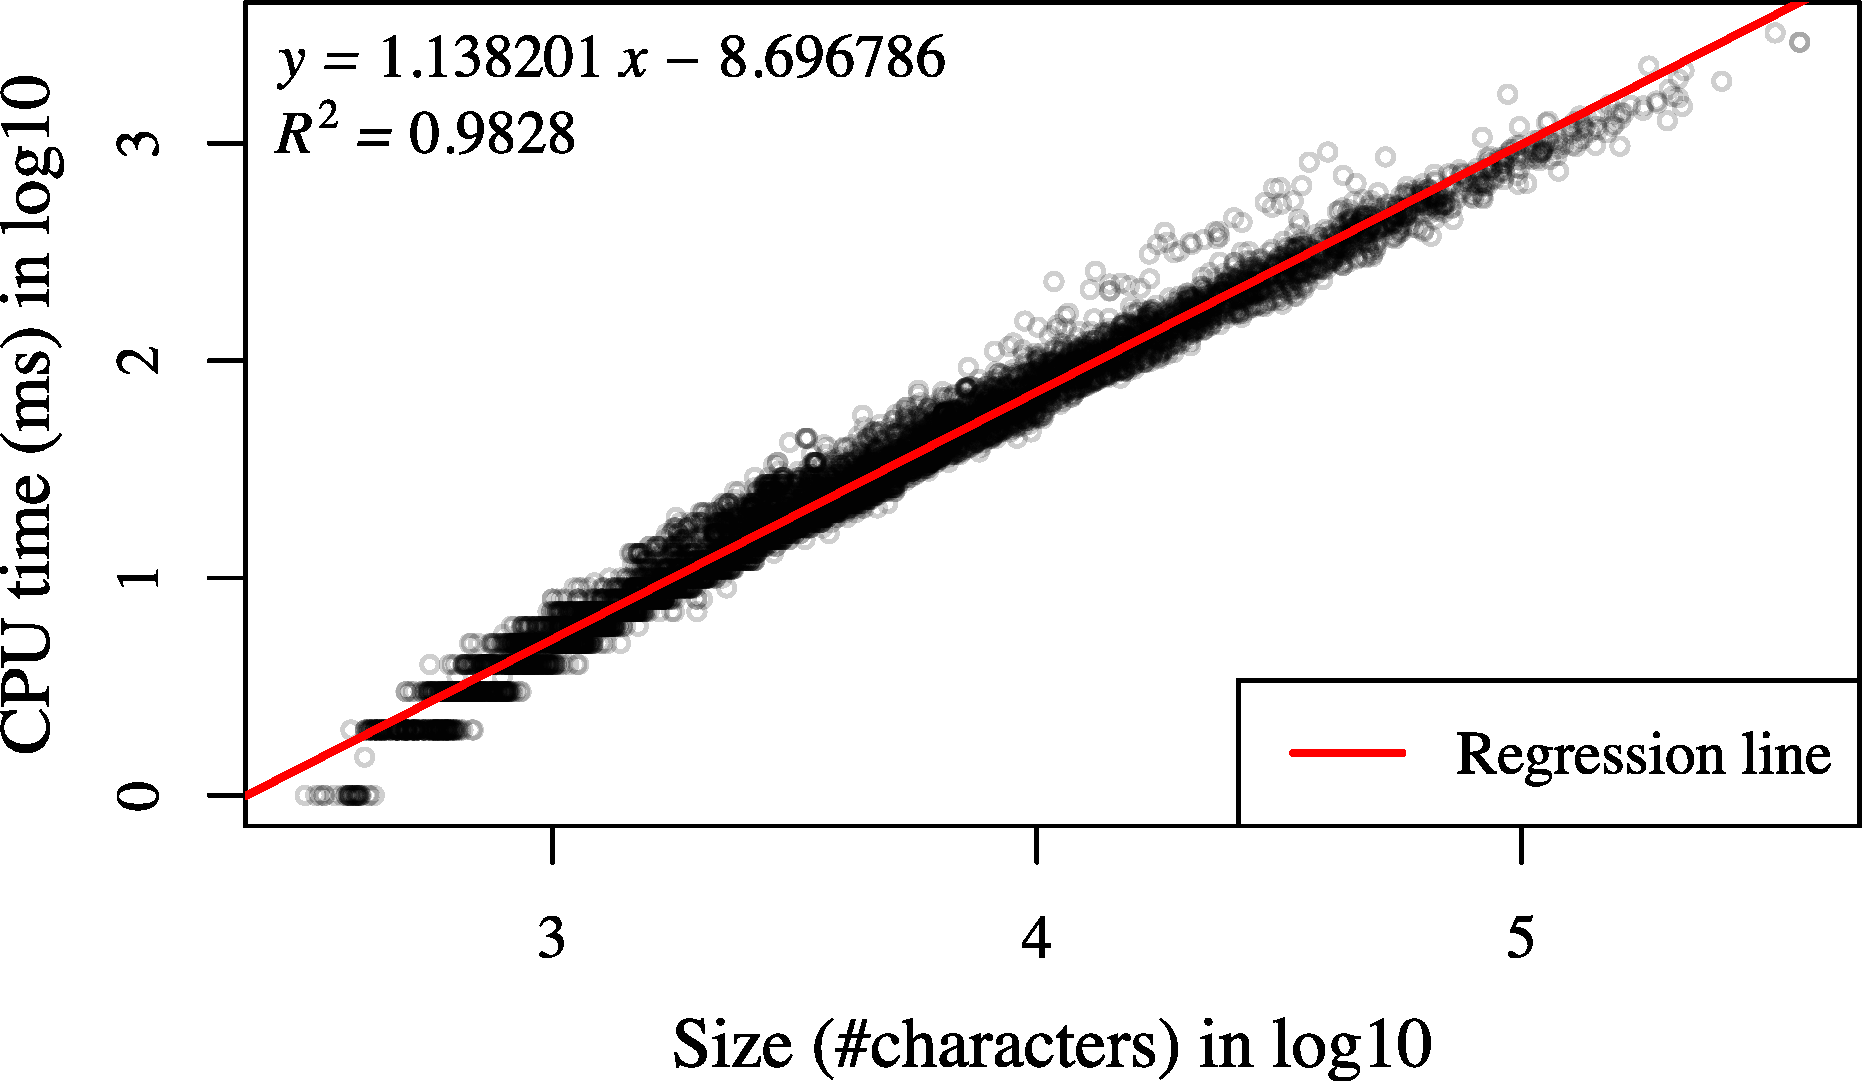
\includegraphics[width=\textwidth]{pictures/meerkatPerformance.pdf}
      \caption{Meerkat performance on Java files\footnotemark}
    \end{figure}
  \end{minipage}  
  \footnotetext{From ``Practical, general parser combinators''}
\end{frame}

\begin{frame}[fragile]
  \frametitle{Summary}  
  \begin{itemize}
    \item ANTLR is a good choice in general case
    \item TreeSitter may be a good choice for incremental parsing
    \item Generalized parsing (GLL, GLR) is mature enough to be a base for real-world parsing tools
    \item Incremental parsing + precise error recovery = nontrivial challenge    
      \begin{itemize}
    \item \href{https://arxiv.org/pdf/1804.07133.pdf}{Don’t Panic! Better, Fewer, Syntax Errors for LR Parsers}
  \end{itemize} 

  \end{itemize}
\end{frame}


\end{document}
